\documentclass[aspectratio=169]{beamer}
\mode<presentation>
\usetheme{Hannover}
\useoutertheme{sidebar}
\usecolortheme{dolphin}

\usepackage{amsmath}
\usepackage{amssymb}
\usepackage{enumerate}


% some bold math symbosl
\newcommand{\Cov}{\mathrm{Cov}}
\newcommand{\Cor}{\mathrm{Cor}}
\newcommand{\Var}{\mathrm{Var}}
\newcommand{\brho}{\boldsymbol{\rho}}
\newcommand{\bSigma}{\boldsymbol{\Sigma}}
\newcommand{\btheta}{\boldsymbol{\theta}}
\newcommand{\bbeta}{\boldsymbol{\beta}}
\newcommand{\bmu}{\boldsymbol{\mu}}
\newcommand{\bW}{\mathbf{W}}
\newcommand{\one}{\mathbf{1}}
\newcommand{\bH}{\mathbf{H}}
\newcommand{\by}{\mathbf{y}}
\newcommand{\bolde}{\mathbf{e}}
\newcommand{\bx}{\mathbf{x}}

\newcommand{\cpp}[1]{\texttt{#1}}

\title{Mathematical Biostatistics Boot Camp: Lecture 13, Binomial Proportions}
\author{Brian Caffo}
\date{\today}
\institute[Department of Biostatistics]{
  Department of Biostatistics \\
  Johns Hopkins Bloomberg School of Public Health\\
  Johns Hopkins University
}


\begin{document}

\frame{\titlepage}


\section{Table of contents}
\frame{
  \frametitle{Table of contents}
  \tableofcontents
}

\section{Intervals for binomial proportions}
\begin{frame}\frametitle{Intervals for binomial parameters}
\begin{itemize}
\item When $X\sim\mbox{Binomial}(n, p)$ we know that
  \begin{enumerate}[a.]
  \item $\hat p = X / n$ is the MLE for $p$
  \item $E[\hat p] = p$
  \item $\Var(\hat p) = p (1 - p) / n$
  \item $
        \frac{\hat p - p}{\sqrt{\hat p (1- \hat p)/n}}
         $
  follows a normal distribution for large $n$
  \end{enumerate}
\item The latter fact leads to the Wald interval for $p$
  $$
  \hat p \pm Z_{1-\alpha/2} \sqrt{\hat p (1 - \hat p) / n}
  $$
\end{itemize}
\end{frame}
 
\begin{frame}\frametitle{Some discussion}
\begin{itemize}
\item The Wald interval performs terribly
\item Coverage probability varies wildly, sometimes being quite low for 
  certain values of $n$ even when $p$ is not near the boundaries
  \begin{itemize}
  \item Example, when $p=.5$ and $n=40$ the actual coverage of a $95\%$ interval
    is only $92\%$
  \end{itemize}
\item When $p$ is small or large, coverage can be quite poor even for extremely
  large values of $n$
  \begin{itemize}
  \item Example, when $p=.005$ and $n=1,876$ the actual coverage rate of a $95\%$
    interval is only $90\%$
  \end{itemize}
\end{itemize}
\end{frame}

\section{Agresti- Coull interval}
\begin{frame}\frametitle{Simple fix}
\begin{itemize}
\item A simple fix for the problem is to add two successes and two failures
\item That is let $\tilde p = (X + 2) / (n + 4)$
\item The (Agresti- Coull) interval is 
  $$
  \tilde p \pm Z_{1-\alpha/2} \sqrt{\tilde p (1 - \tilde p) / \tilde n}
  $$
\item Motivation: when $p$ is large or small, the distribution of
  $\hat p$ is skewed and it does not make sense to center the interval
  at the MLE; adding the pseudo observations pulls the center of
  the interval toward $.5$
\item Later we will show that this interval is the inversion of a
  hypothesis testing technique
\end{itemize}
\end{frame}

\begin{frame}\frametitle{Example}
Suppose that in a random sample of an at-risk population
$13$ of $20$ subjects had hypertension. Estimate the prevalence
of hypertension in this population.
\begin{itemize}
\item $\hat p = .65$,  $n = 20$
\item $\tilde p = .63$, $\tilde n = 24$
\item $Z_{.975} = 1.96$
\item Wald interval $[.44, .86]$
\item Agresti-Coull interval $[.44, .82]$ 
\item $1/8$ likelihood interval $[.42, .84]$
\end{itemize}
\end{frame}

\begin{frame}
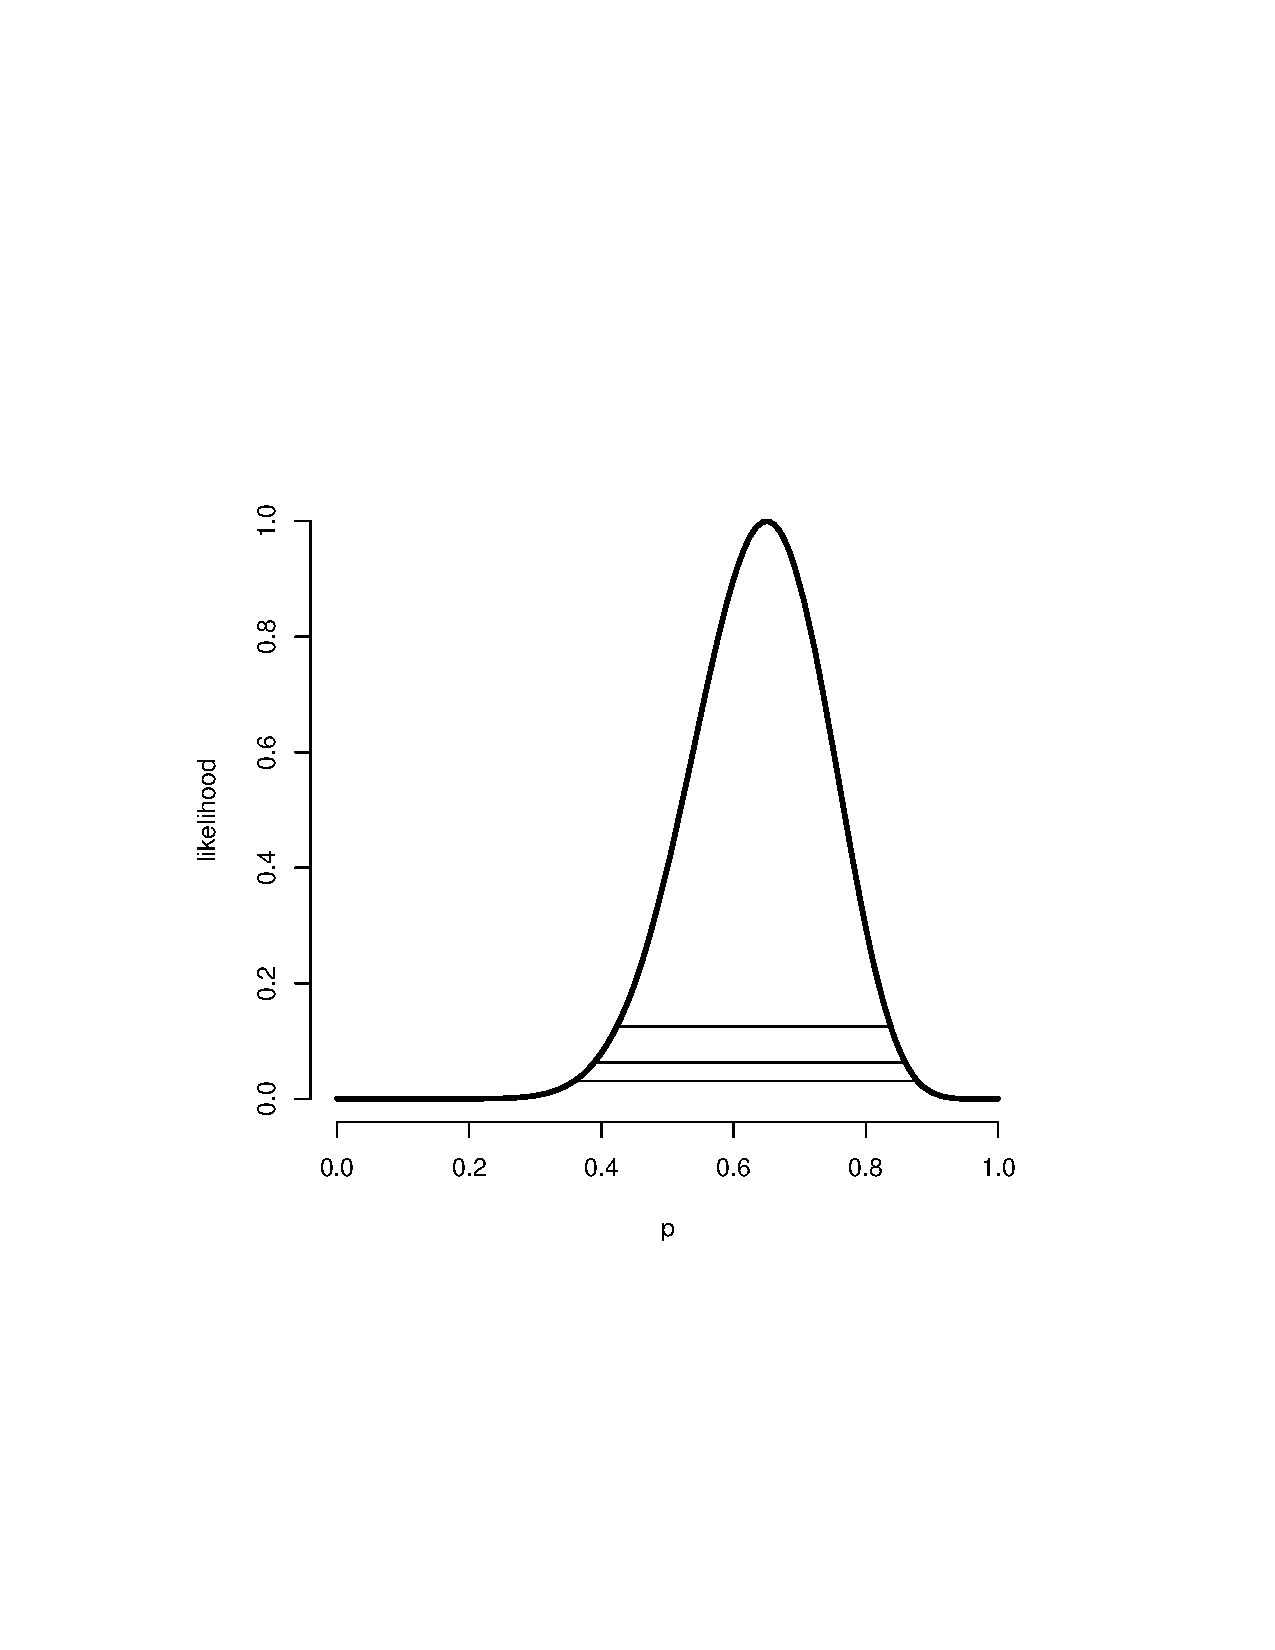
\includegraphics[width=3.5in]{binomialLikelihoodExample.pdf}
\end{frame}

\section{Bayesian analysis}
\begin{frame}\frametitle{Bayesian analysis}
\begin{itemize}
\item Bayesian statistics posits a {\bf prior} on the parameter
  of interest
\item All inferences are then performed on the distribution of 
  the parameter given the data, called the {\bf posterior}
\item In general,
  $$
  \mbox{Posterior} \propto \mbox{Likelihood} \times \mbox{Prior}
  $$
\item Therefore (as we saw in diagnostic testing) the likelihood is
  the factor by which our prior beliefs are updated to produce
  conclusions in the light of the data
\end{itemize}
\end{frame}

\subsection{Prior specification}
\begin{frame}\frametitle{Beta priors}
\begin{itemize}
\item The beta distribution is the default prior
  for parameters between $0$ and $1$.
\item The beta density depends on two parameters $\alpha$ and $\beta$
$$
\frac{\Gamma(\alpha +  \beta)}{\Gamma(\alpha)\Gamma(\beta)}
 p ^ {\alpha - 1} (1 - p) ^ {\beta - 1} ~~~~\mbox{for} ~~ 0 \leq p \leq 1
$$
\item The mean of the beta density is $\alpha / (\alpha + \beta)$
\item The variance of the beta density is \
$$\frac{\alpha \beta}{(\alpha + \beta)^2 (\alpha + \beta + 1)}$$
\item The uniform density is the special case where $\alpha = \beta = 1$
\end{itemize}
\end{frame}

\begin{frame}
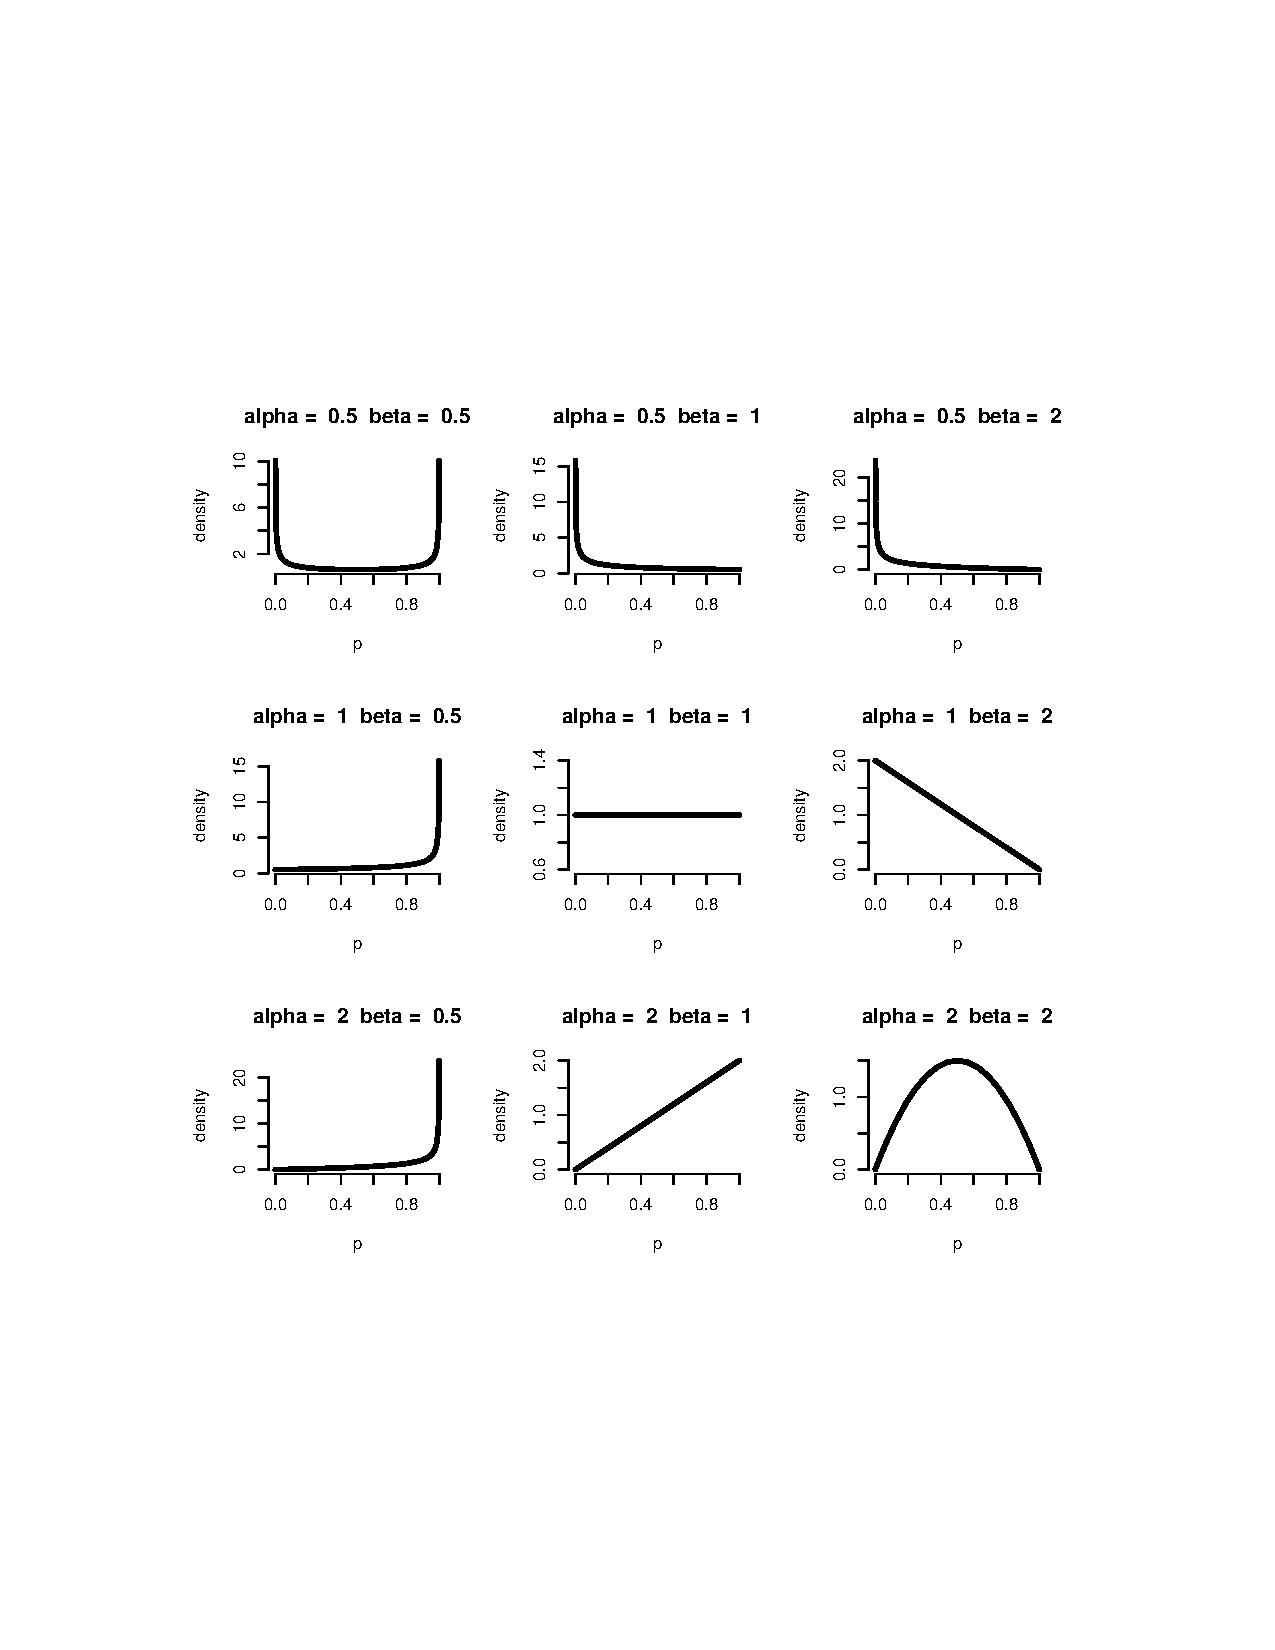
\includegraphics[width=3.5in]{beta.pdf}
\end{frame}

\subsection{Posterior}
\begin{frame}\frametitle{Posterior}
\begin{itemize}
\item Suppose that we chose values of $\alpha$ and $\beta$ so that
  the beta prior is indicative of our degree of belief regarding $p$
  in the absence of data
\item Then using the rule that
  $$
  \mbox{Posterior} \propto \mbox{Likelihood} \times \mbox{Prior}
  $$
  and throwing out anything that doesn't depend on $p$, we have that
\begin{eqnarray*}
\mbox{Posterior} &\propto & p^x(1 - p)^{n-x} \times p^{\alpha -1} (1 - p)^{\beta - 1} \\
                 &  =     & p^{x + \alpha - 1} (1 - p)^{n - x + \beta - 1}
\end{eqnarray*}
\item This density is just another beta density with parameters
  $\tilde \alpha = x + \alpha$ and $\tilde \beta = n - x + \beta$
\end{itemize}
\end{frame}

\begin{frame}\frametitle{Posterior mean}
\begin{itemize}
\item Posterior mean 
 \begin{eqnarray*}
E[p ~|~ X] & = &  \frac{\tilde \alpha}{\tilde \alpha + \tilde \beta}\\ \\
& = & \frac{x + \alpha}{x + \alpha + n - x + \beta}\\ \\
& = & \frac{x + \alpha}{n + \alpha + \beta} \\ \\
& = & \frac{x}{n} \times \frac{n}{n + \alpha + \beta} + \frac{\alpha}{\alpha + \beta} \times \frac{\alpha + \beta}{n + \alpha + \beta} \\ \\
& = & \mbox{MLE} \times \pi + \mbox{Prior Mean} \times (1 - \pi)
  \end{eqnarray*}
\end{itemize}
\end{frame}


\begin{frame}
\begin{itemize}
\item The posterior mean is a mixture of the MLE ($\hat p$) and the
  prior mean
\item $\pi$ goes to $1$ as $n$ gets large; for large $n$ the data swamps the prior
\item For small $n$, the prior mean dominates 
\item Generalizes how science should ideally work; as data becomes
  increasingly available, prior beliefs should matter less and less
\item With a prior that is degenerate at a value, no amount of data
  can overcome the prior
\end{itemize}
\end{frame}

\begin{frame}\frametitle{Posterior variance}
\begin{itemize}
\item The posterior variance is
  \begin{eqnarray*}
\Var(p ~|~ x) & = & \frac{\tilde \alpha \tilde \beta}%
{(\tilde \alpha + \tilde \beta)^2 (\tilde \alpha + \tilde \beta + 1)} \\ \\
& = & 
\frac{ (x + \alpha)(n - x + \beta)}%
{(n + \alpha + \beta)^2 (n + \alpha + \beta + 1)}
\end{eqnarray*}
\item Let $\tilde p = (x + \alpha) / (n + \alpha + \beta)$ and $\tilde n = n + \alpha + \beta$ then we have
$$
\Var(p ~|~ x) = \frac{\tilde p (1 - \tilde p)}{\tilde n + 1}
$$
\end{itemize}
\end{frame}

\begin{frame}\frametitle{Discussion}
\begin{itemize}
\item If $\alpha = \beta = 2$ then the posterior mean is
$$
\tilde p = (x + 2) / (n + 4)
$$
and the posterior variance is 
$$
\tilde p (1 - \tilde p) / (\tilde n + 1)
$$
\item This is almost exactly the mean and variance we used for
  the Agresti-Coull interval
\end{itemize}
\end{frame}

\begin{frame}\frametitle{Example}
\begin{itemize}
\item Consider the previous example where $x = 13$ and $n=20$
\item Consider a uniform prior, $\alpha = \beta = 1$
\item The posterior is proportional to (see formula above)
$$
p^{x + \alpha - 1} (1 - p)^{n - x + \beta - 1} = p^x (1 - p)^{n-x}
$$
that is, for the uniform prior, the posterior is the likelihood
\item Consider the instance where $\alpha = \beta = 2$ (recall this prior
is humped around the point $.5$) the posterior is
$$
p^{x + \alpha - 1} (1 - p)^{n - x + \beta - 1} = p^{x + 1} (1 - p)^{n-x + 1}
$$
\item The ``Jeffrey's prior'' which has some theoretical benefits
  puts $\alpha = \beta = .5$
\end{itemize}
\end{frame}


\begin{frame}
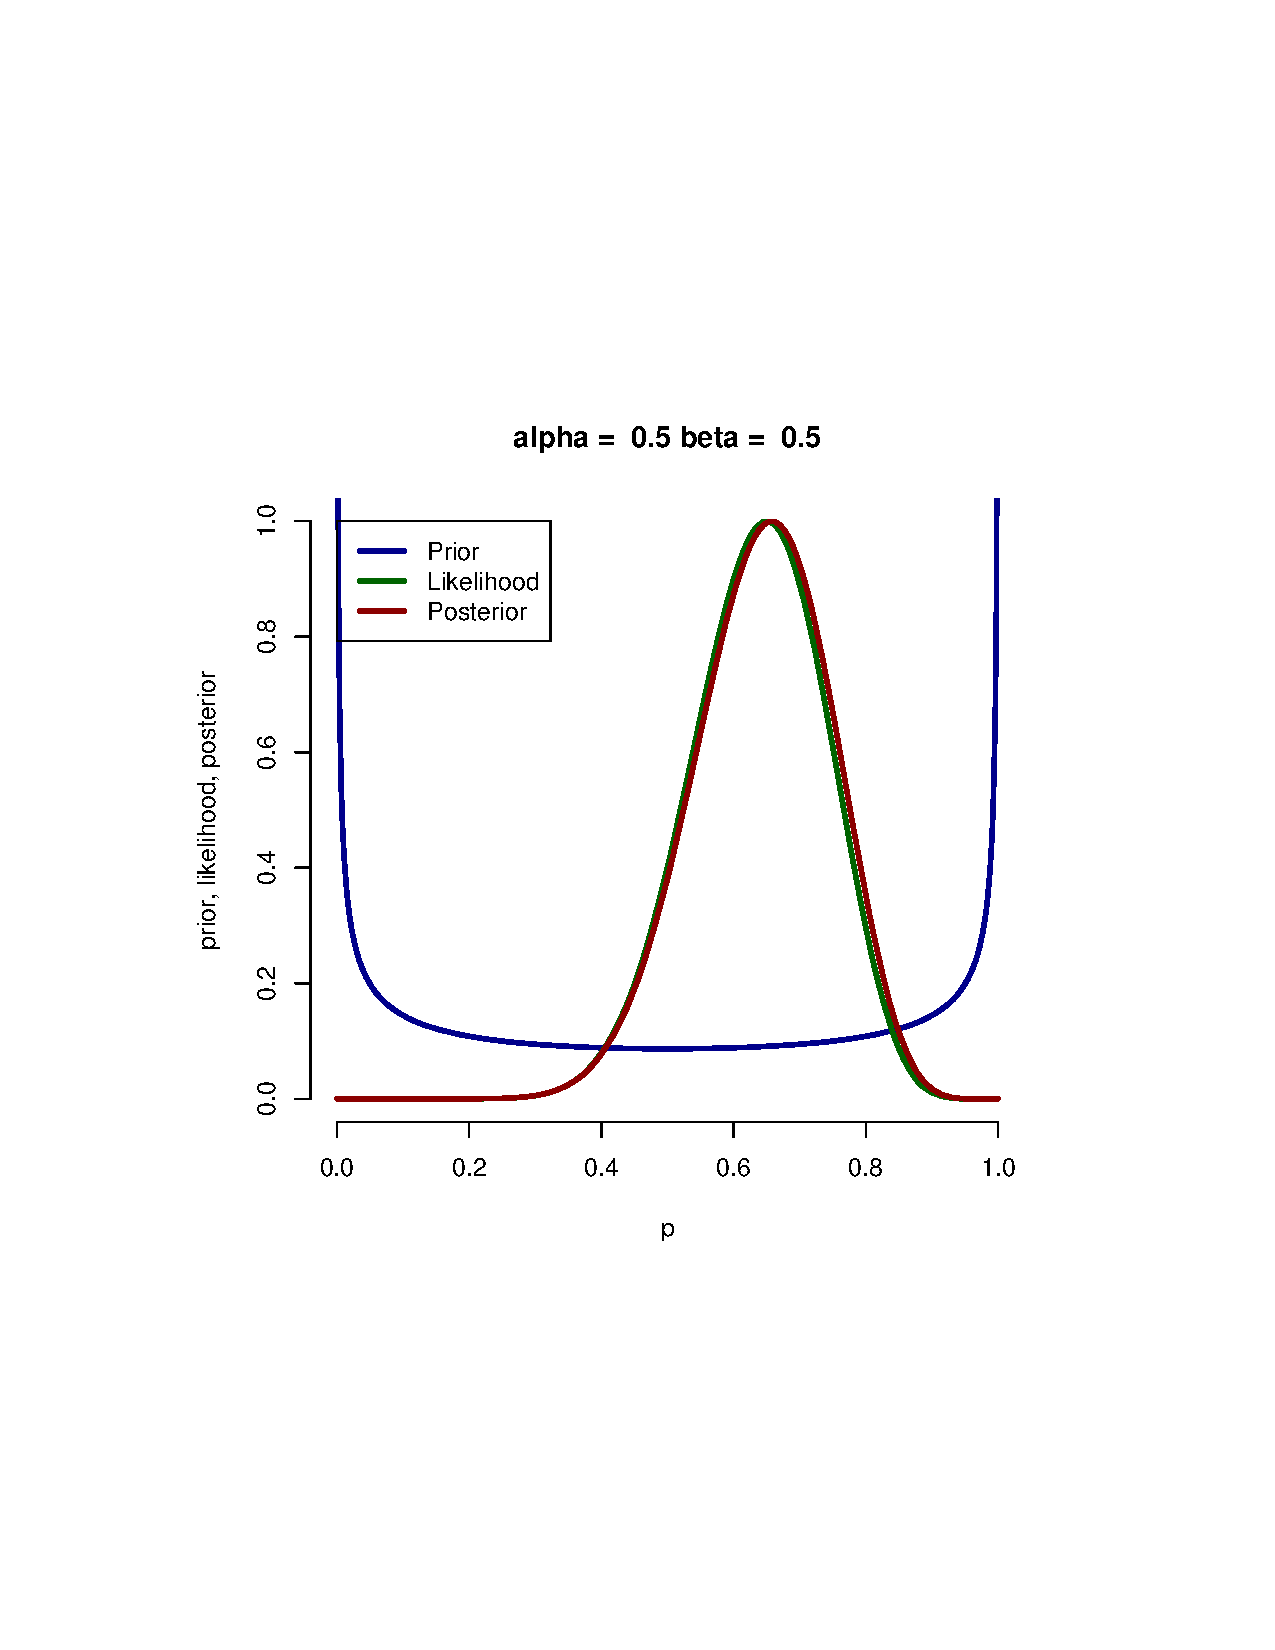
\includegraphics[width=3.5in]{binBayes1.pdf}
\end{frame}

\begin{frame}
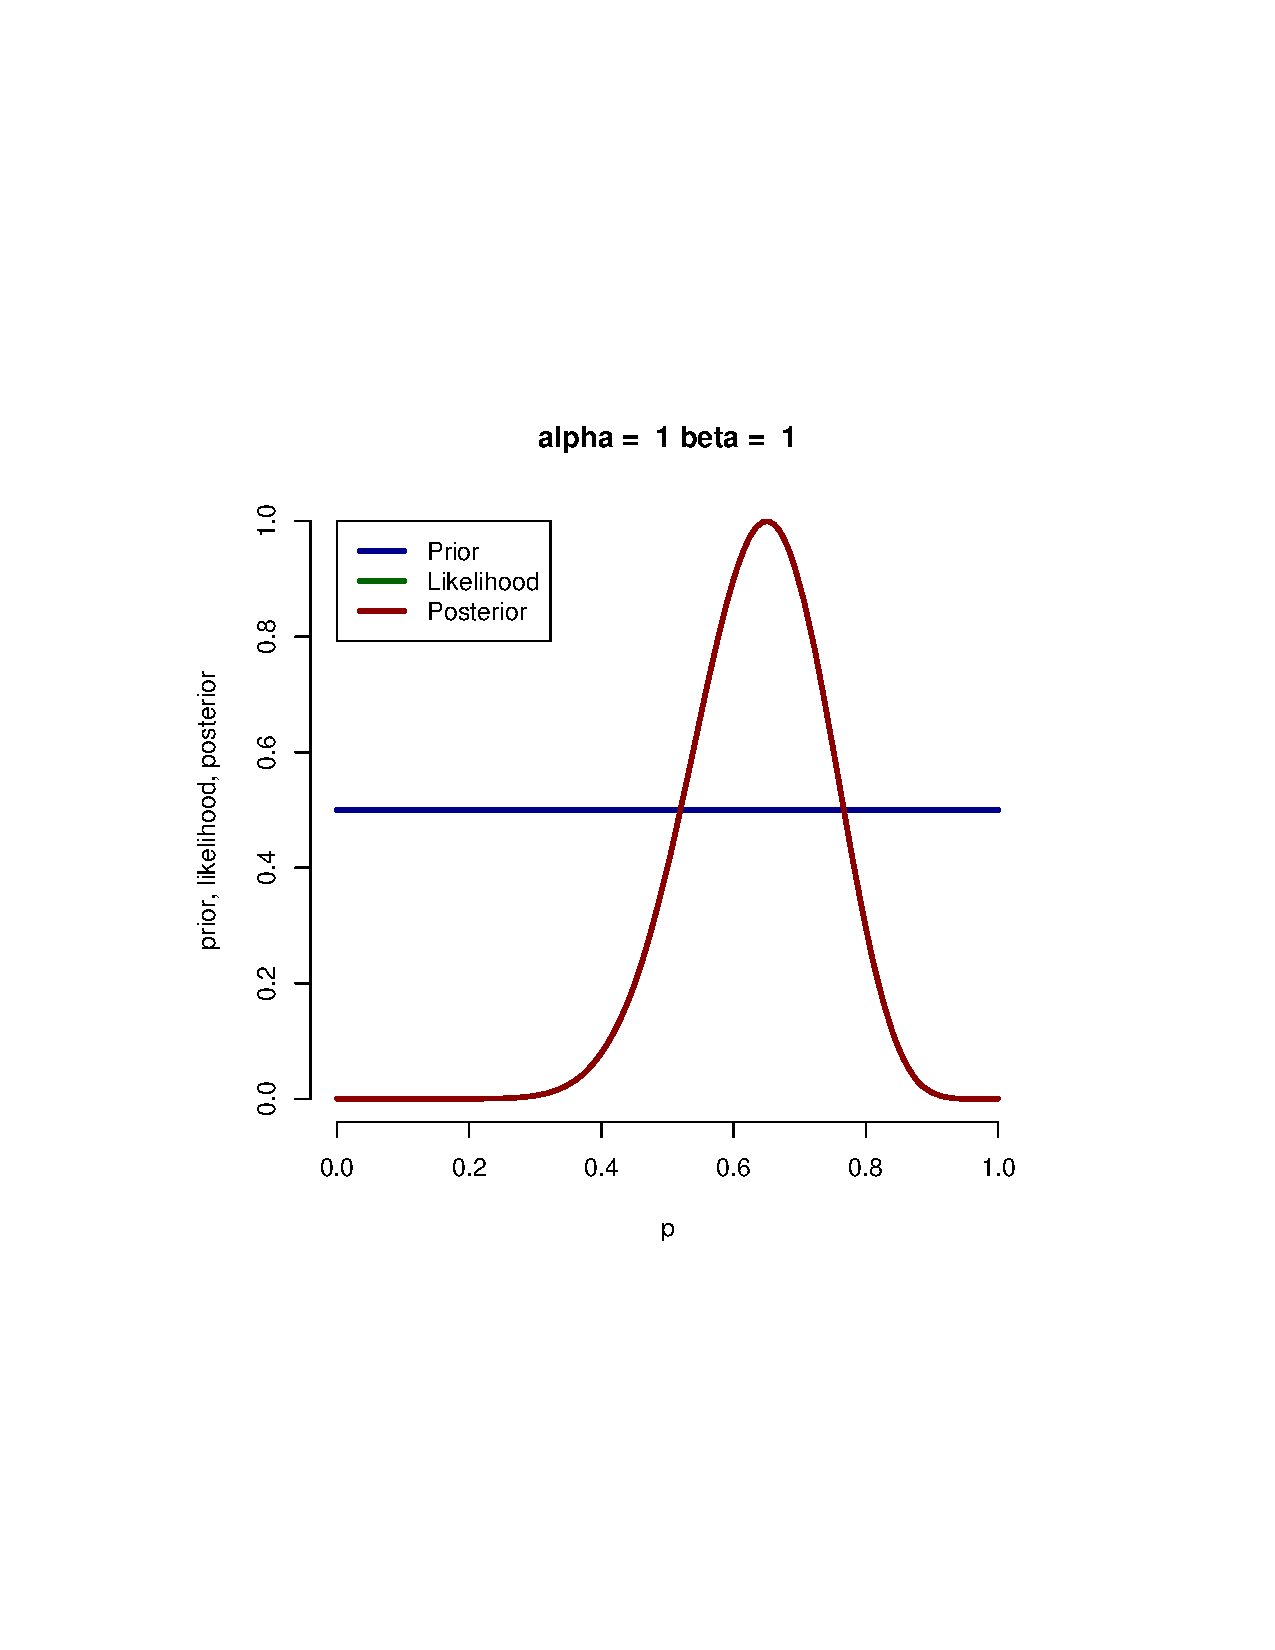
\includegraphics[width=3.5in]{binBayes2.pdf}
\end{frame}

\begin{frame}
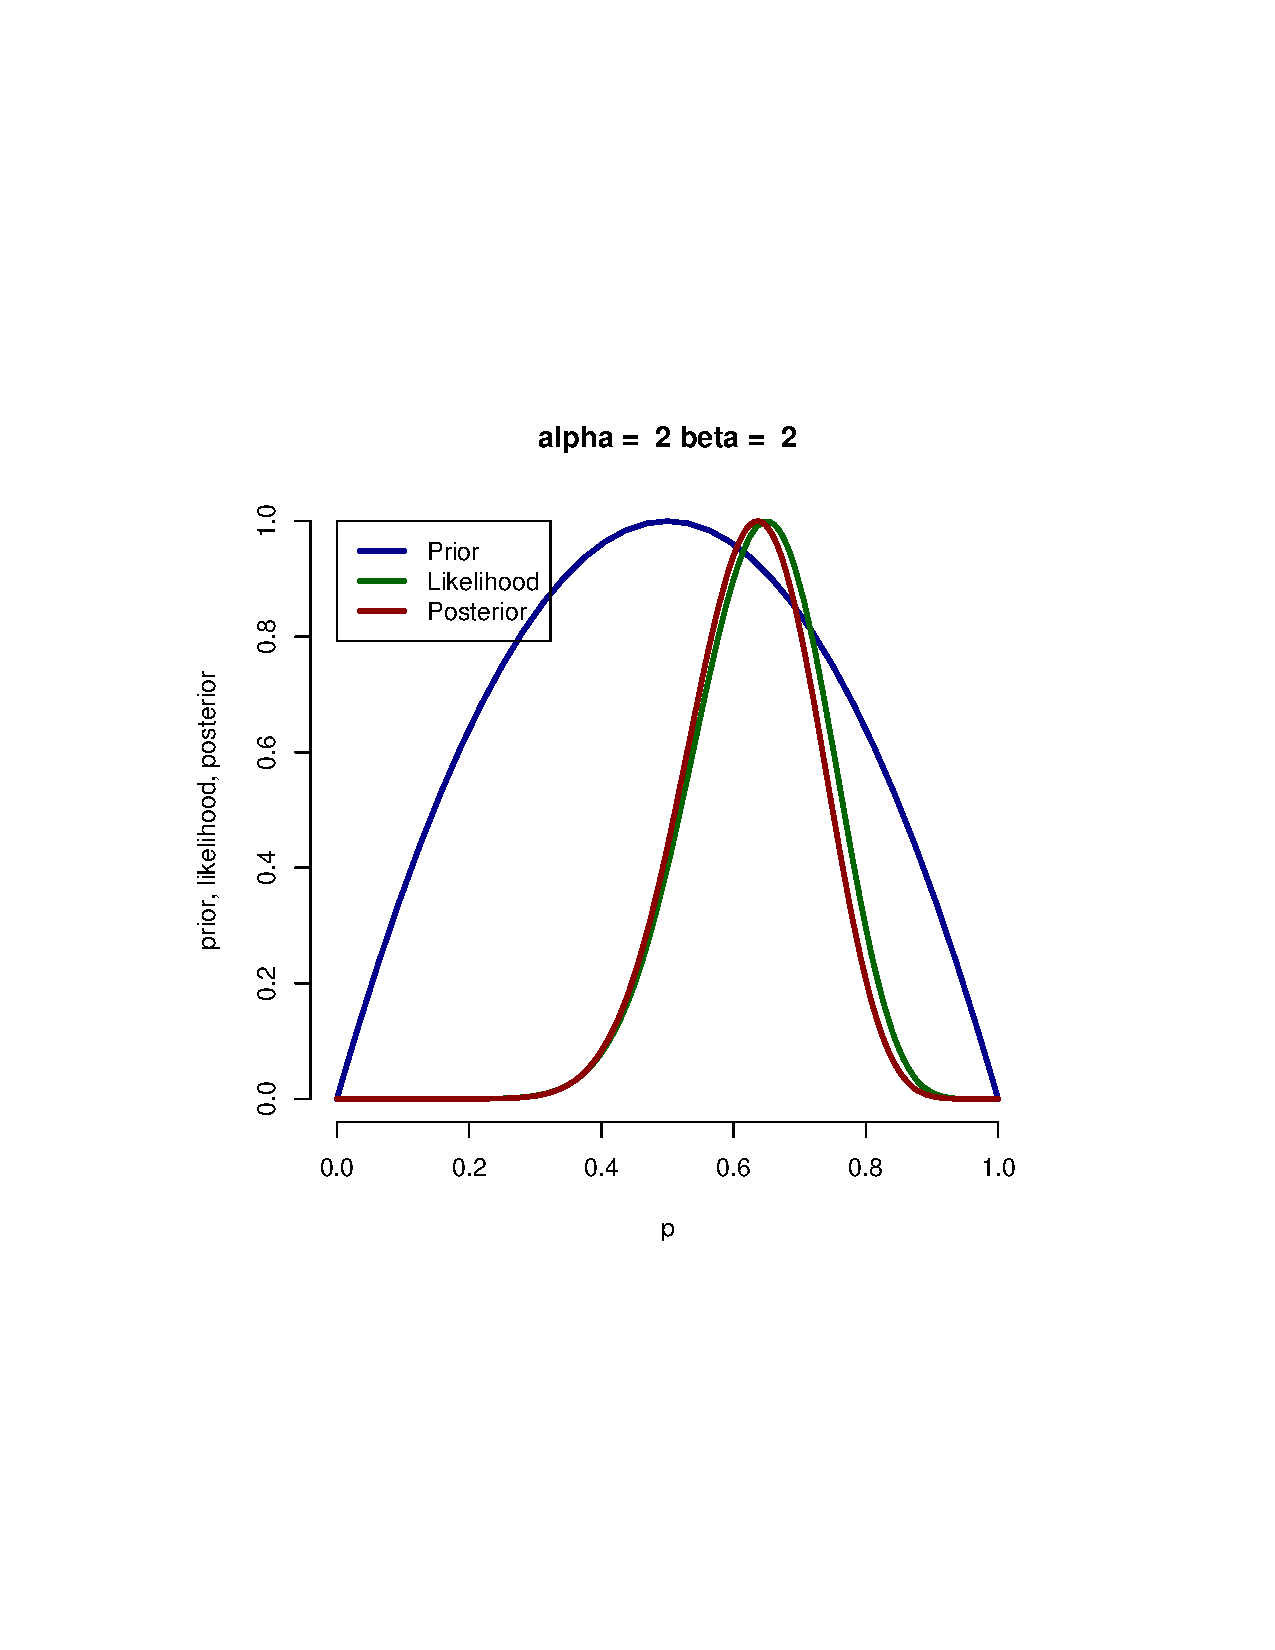
\includegraphics[width=3.5in]{binBayes3.pdf}
\end{frame}

\begin{frame}
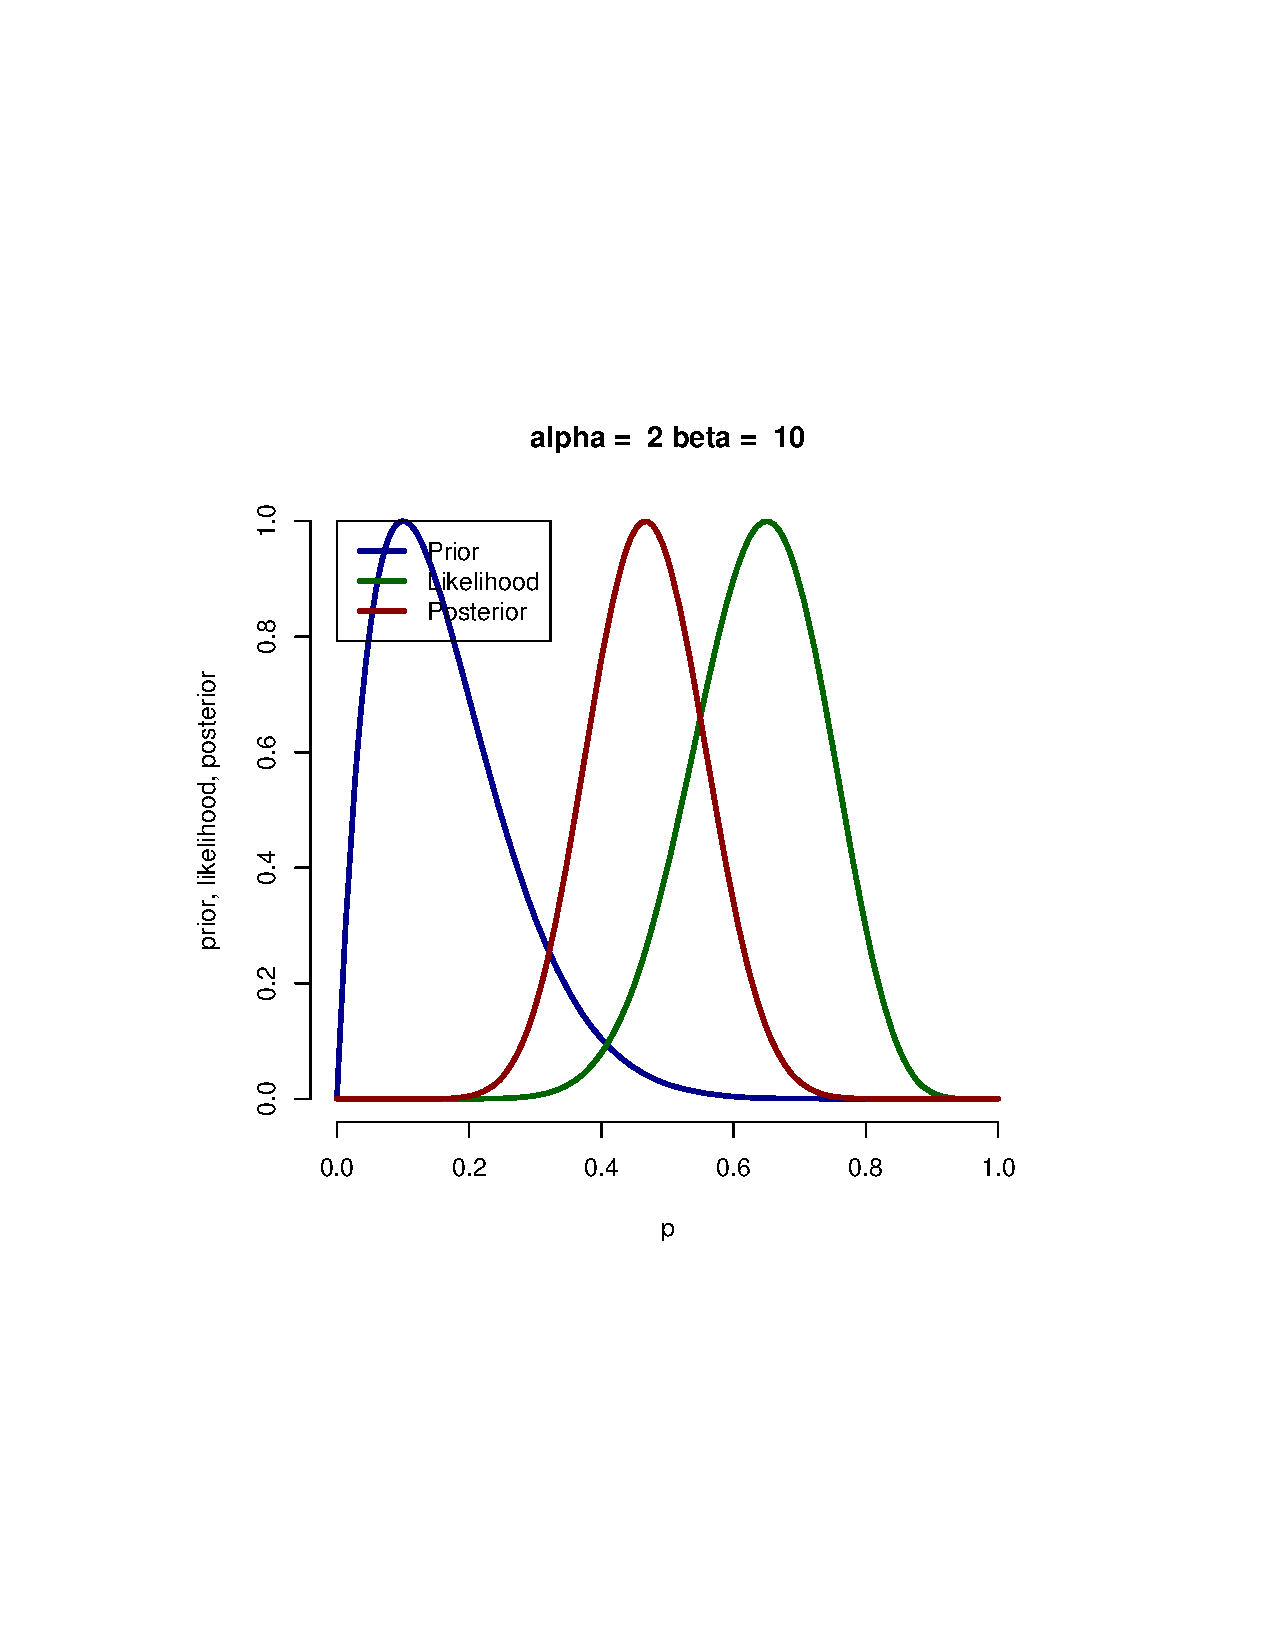
\includegraphics[width=3.5in]{binBayes4.pdf}
\end{frame}

\begin{frame}
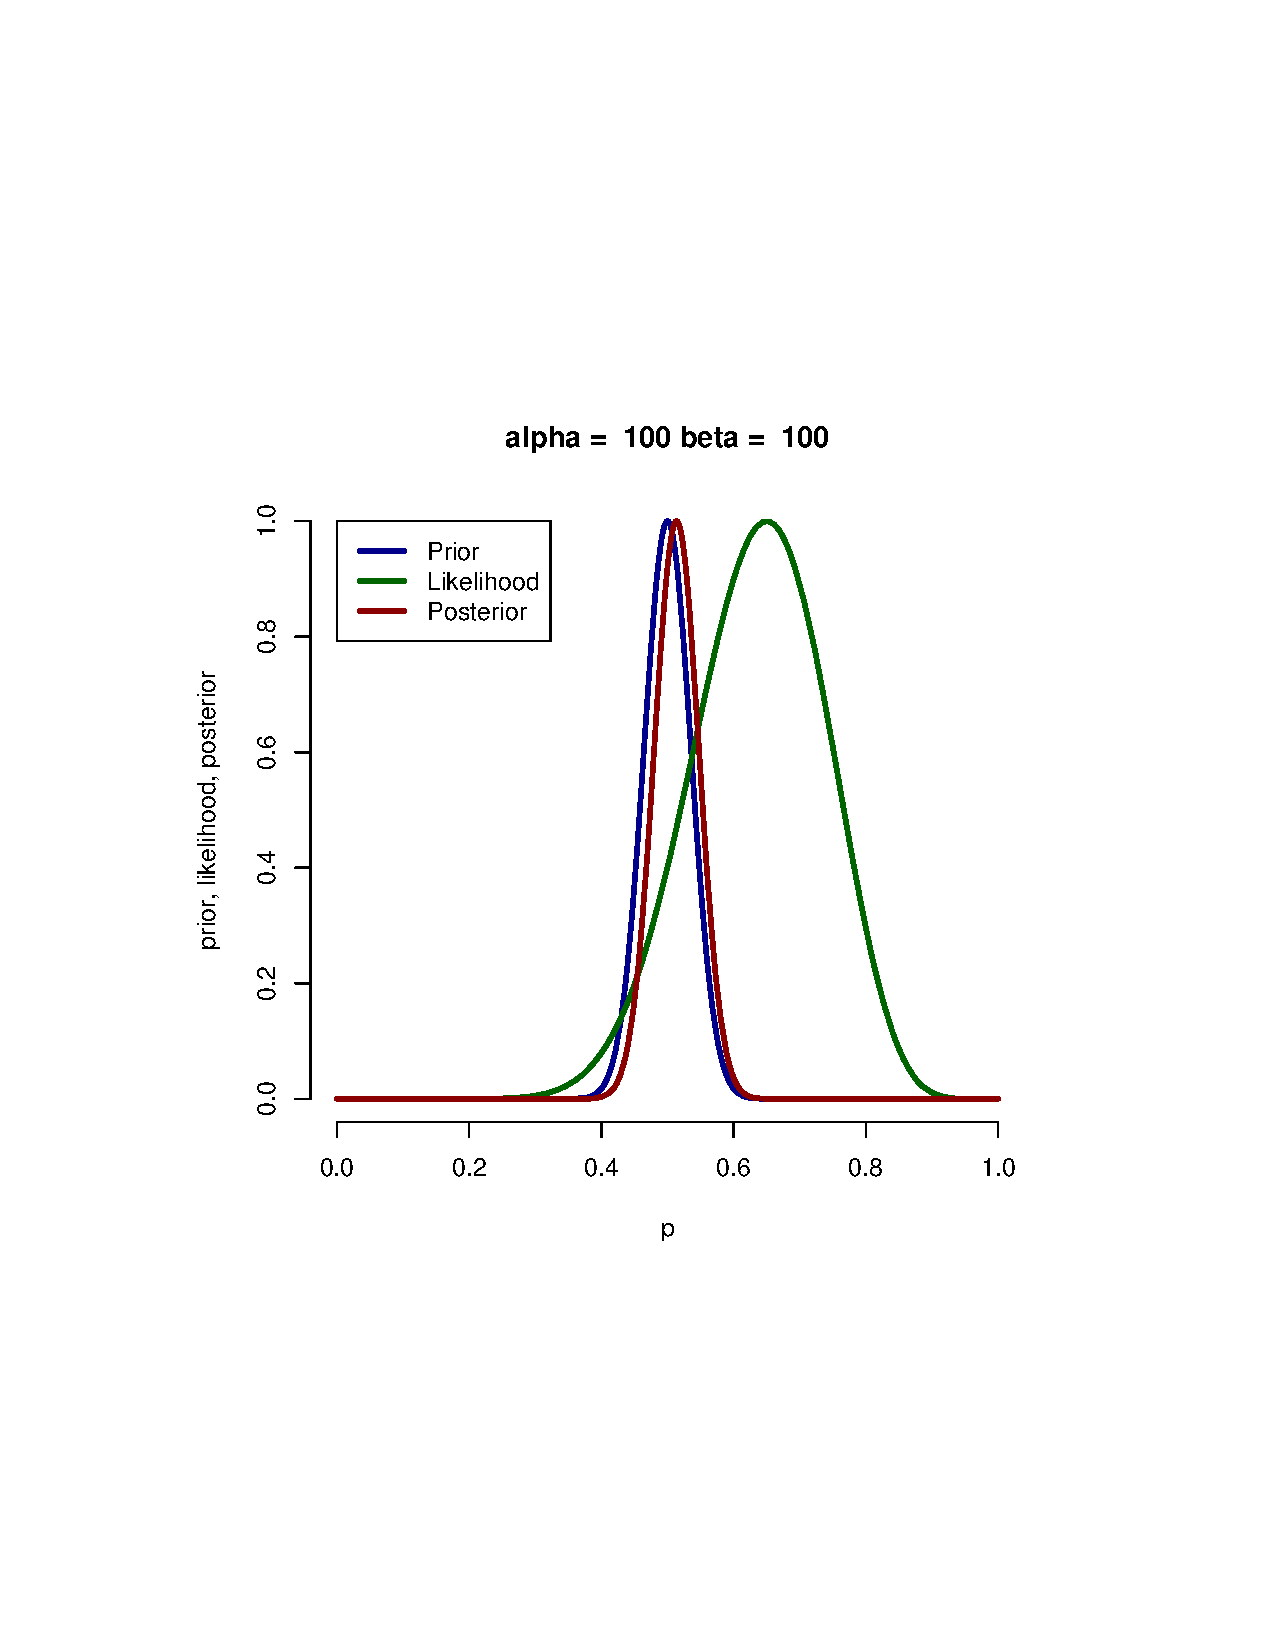
\includegraphics[width=3.5in]{binBayes5.pdf}
\end{frame}

\subsection{Credible intervals}
\begin{frame}\frametitle{Bayesian credible intervals}
\begin{itemize}
\item A {\em Bayesian credible interval} is the  Bayesian analog of a confidence
  interval
\item A $95\%$ credible interval, $[a, b]$ would satisfy
  $$
  P(p \in [a, b] ~|~ x) = .95
  $$
\item The best credible intervals chop off the posterior with a horizontal
  line in the same way we did for likelihoods 
\item These are called highest posterior density (HPD) intervals
\end{itemize}
\end{frame}

\begin{frame}
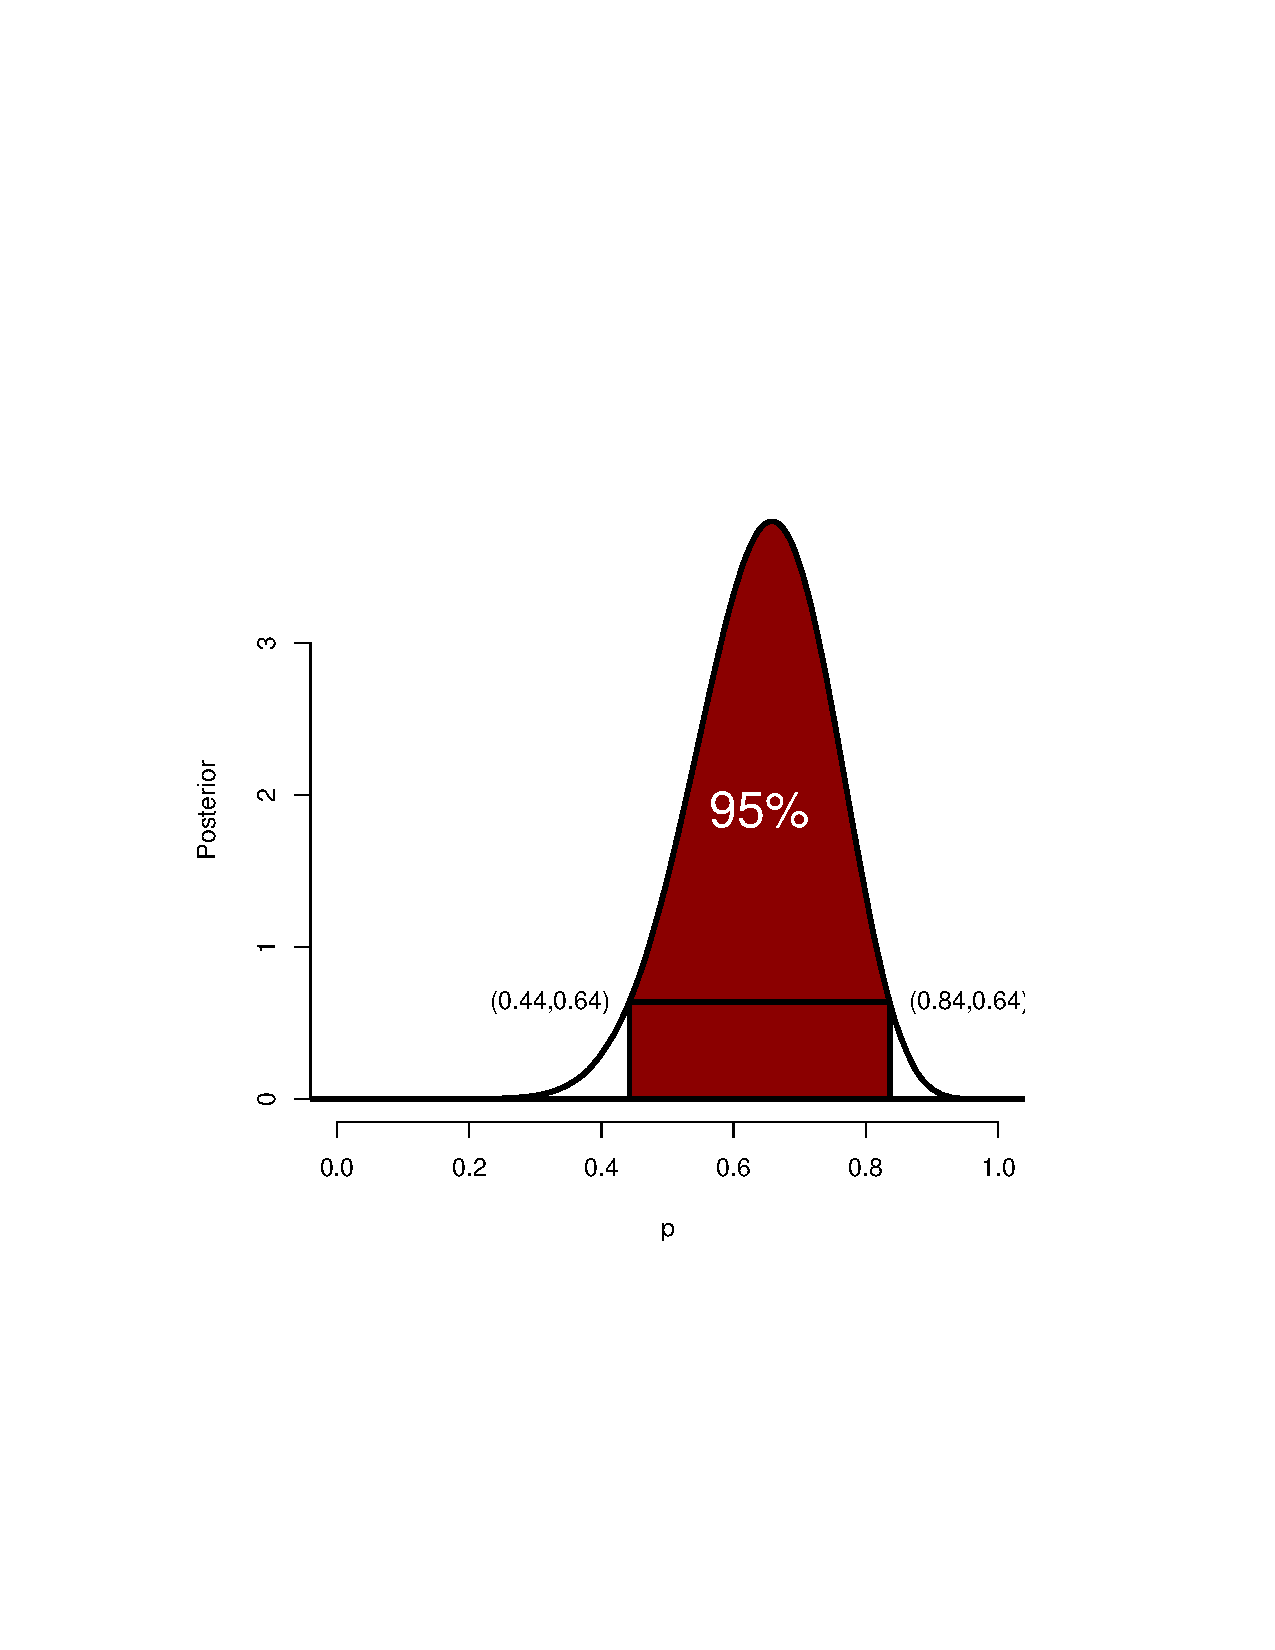
\includegraphics[width=3.5in]{hpd.pdf}
\end{frame}


\begin{frame}[fragile]\frametitle{R code}
Install the \texttt{binom} package, then the command
\begin{verbatim}
library(binom)
binom.bayes(13, 20, type = "highest")
\end{verbatim}
gives the HPD interval. The default credible level is $95\%$ and
the default prior is the Jeffrey's prior.
\end{frame}

\begin{frame}\frametitle{Interpretation of confidence intervals}
\begin{itemize}
\item Confidence interval: (Wald) $[.44, .86]$
\item Fuzzy interpretation: 
  \begin{quote}
We are 95\% confident that $p$ lies between $.44$ to $.86$    
  \end{quote}
\item Actual interpretation: 
  \begin{quote}
    The interval $.44$ to $.86$ was constructed such that in repeated
    independent experiments, $95\%$ of the intervals obtained would
    contain $p$.
  \end{quote}
\item Yikes!
\end{itemize}
\end{frame}

\section{Summary}
\begin{frame}\frametitle{Likelihood intervals}
\begin{itemize}
\item Recall the $1/8$ likelihood interval was $[.42, .84]$
\item Fuzzy interpretation:
  \begin{quote}
    The interval $[.42, .84]$ represents plausible values for $p$.
  \end{quote}
\item Actual interpretation
  \begin{quote}
    The interval $[.42, .84]$ represents plausible values for $p$ in
    the sense that for each point in this interval, there is no
    other point that is more than $8$ times better supported given the data.
  \end{quote}
\item Yikes!
\end{itemize}
\end{frame}

\begin{frame}\frametitle{Credible intervals}
\begin{itemize}
\item Recall the Jeffrey's prior $95\%$ credible interval was \\$[.44, .84]$
\item Actual interpretation
  \begin{quote}
    The probability that $p$ is between $.44$ and $.84$ is $95\%$.
  \end{quote}
\end{itemize}
\end{frame}

\end{document}

